\section{Conditions de mesures}
Pour les mesures de tension et de courants, les roues ont été retirées de la maquette. De cette manière, le \Gls{pcb} était facilement accessible.

Pour les mesures embarquées, la période de mesure $T_{mes}$ du module est fixée à 20 ms.
\subsection{Appareils de mesure}

\begin{table}[H]
    \centering
    \begin{tabular}{|l|l|l|}
        \hline
        \textbf{Type} & \textbf{Marque} & \textbf{Modèle} \\
        \hline
        Multimètre numérique & UNI-T & UT61E \\
        \hline
    \end{tabular}
    \caption{Appareils de mesure}
    \label{tab:appareils_mesure}
\end{table}

\section{Modèle physique}

Configuration PID : $K_{pv}=26$, $K_{pt}=1.53$, $T_{dt}=0.38$.

Les paramètres $K_{pv}$ et $K_{pt}$ correspondent respectivement aux gains proportionnels de la boucle de vitesse et de la boucle d'inclinaison, tandis que $T_{dt}$ représente la constante du terme dérivé utilisée pour améliorer l'amortissement de la réponse.

Afin de valider le modèle physique développé précédemment, plusieurs essais expérimentaux ont été réalisés puis comparés aux résultats obtenus par simulation. Les essais portent sur les principaux phénomènes dynamiques intervenant lors du fonctionnement du système : la chute libre, les limitations de vitesse et d'angle, la régulation de maintien, le suivi d'une trajectoire trapézoïdale ainsi que l'influence des mesures issues de l'IMU.

L'objectif est de vérifier que le modèle reproduit fidèlement le comportement réel du système et que les hypothèses retenues sont suffisantes pour représenter sa dynamique.


\subsection{Chute libre}

La phase de chute libre correspond à la période durant laquelle le système n'est soumis qu'à l'action de la gravité. Cette phase permet entre autre d'observer l'effet de l'IMU dans la mesure d'angle.

Les conditions initiales utilisées pour les simulations de chute libre sont définies par le vecteur d'état suivant :

$$
\vec{X} = (x,\dot{x},\theta,\dot{\theta})
$$

Pour les deux cas étudiés, les conditions initiales sont les suivantes :

Cas positif :
$$
\vec{X}_0 = (0,0,0.03^\circ,0)
$$

Cas négatif :
$$
\vec{X}_0 = (0,0,-0.015^\circ,0)
$$

Les figures \ref{fig:chute_libre_positif} et \ref{fig:chute_libre_negatif} présentent l'évolution des grandeurs cinématiques lors d'une chute libre pour deux orientations initiales différentes : un angle positif et un angle négatif.

Dans le cas d'un angle positif (figure \ref{fig:chute_libre_positif}), le système présente une évolution correspondant au mouvement attendu sous l'effet de la gravité. La vitesse angulaire augmente à mesure que le châssis "tombe", tandis que l'orientation évolue selon le mouvement de rotation induit par la configuration initiale.



\begin{figure}[H]
    \centering
    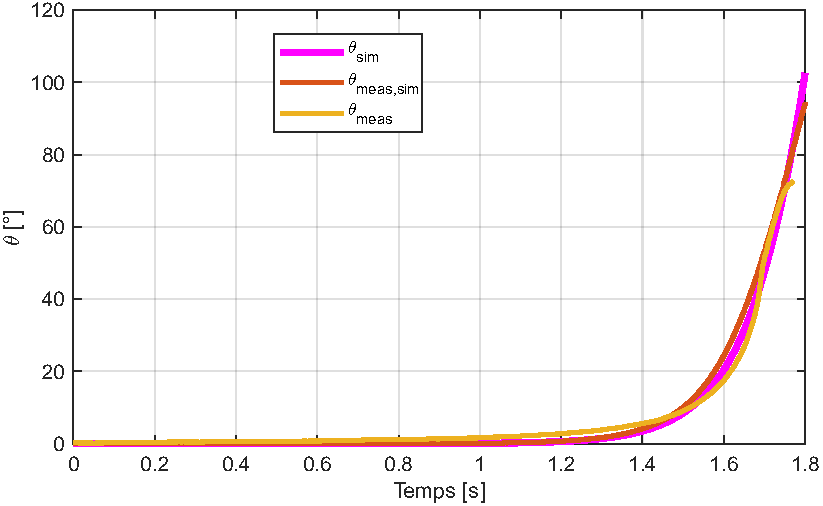
\includegraphics[width=1\textwidth]{assets/figures/graphs/free_fall_positive.pdf}
    \caption{Chute libre, angle positif}
    \label{fig:chute_libre_positif}
\end{figure}

La figure \ref{fig:chute_libre_negatif} présente le comportement obtenu lorsque l'angle initial est inversé. Le changement de signe de l'orientation permet de vérifier la symétrie du modèle et l'influence de la condition initiale sur la dynamique du système.

\begin{figure}[H]
    \centering
    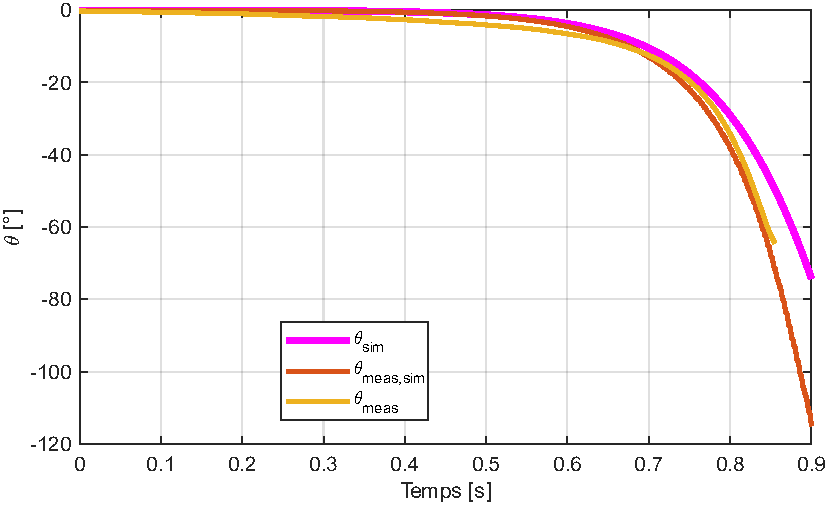
\includegraphics[width=1\textwidth]{assets/figures/graphs/free_fall_negative.pdf}
    \caption{Chute libre, angle négatif}
    \label{fig:chute_libre_negatif}
\end{figure}

Les courbes expérimentales présentent une concordance avec les courbes simulées. Il existe une symmétrie entre les angles négatifs et positifs.

La différence notable est le fait que la courbe théorique "diminue" ou "augmente" plus rapidement que la mesure. 
\subsection{Vitesse maximale}

La vitesse maximale est limitée par le logiciel de commande afin de garantir un fonctionnement sûr du système et d'éviter le dépassement des capacités des moteurs. Pour valider cette limitation, la maquette est maintenue hors de contact du sol puis légèrement inclinée. Cette inclinaison génère une consigne de vitesse qui augmente progressivement jusqu'à atteindre la valeur de saturation programmée.

La figure \ref{fig:max_speed} présente l'évolution de la vitesse mesurée au cours de cet essai. La vitesse (absolue) augmente jusqu'à atteindre une valeur maximale de $0.864\,\mathrm{m/s}$, puis reste limitée à cette valeur.

\begin{figure}[H]
    \centering
    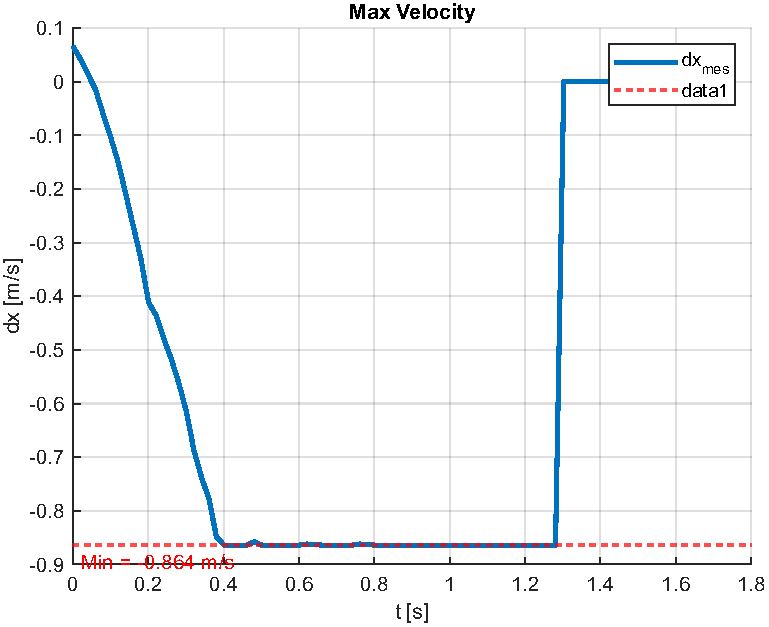
\includegraphics[width=1\textwidth]{assets/figures/graphs/max_speed.pdf}
    \caption{Vitesse maximale mesurée}
    \label{fig:max_speed}
\end{figure}
\subsection{Angle maximal}

Une limite d'inclinaison est implémentée dans le logiciel afin de protéger le système contre une chute ou un fonctionnement en dehors de sa plage de stabilité. Lorsque cette limite est atteinte, la commande coupe immédiatement les moteurs. (voir \ref{chap:developpement_embarque})

La figure \ref{fig:max_angle} présente l'évolution de l'angle d'inclinaison ainsi que de la vitesse du système au cours de l'essai. On observe que lorsque l'angle atteint la valeur limite de $30^\circ$, la vitesse chute instantanément à $0\,\mathrm{m/s}$, traduisant l'arrêt des moteurs.

\begin{figure}[H]
    \centering
    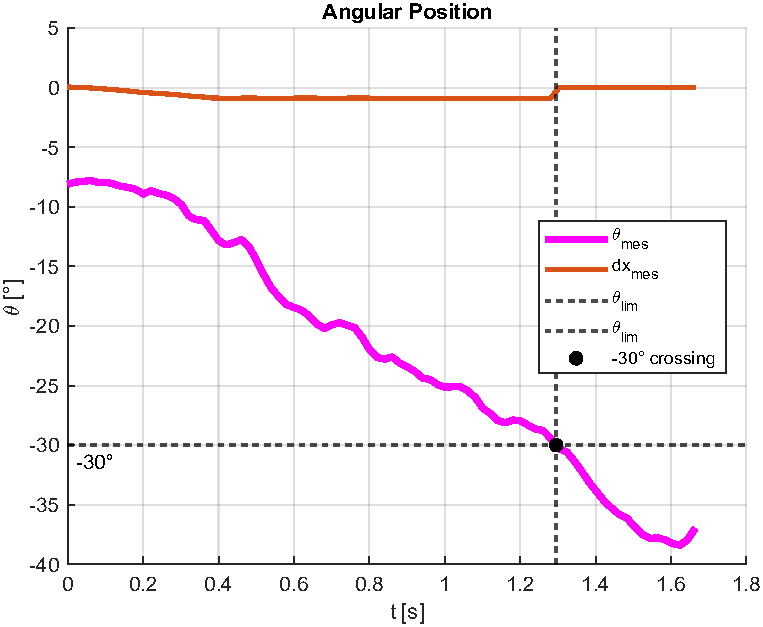
\includegraphics[width=1\textwidth]{assets/figures/graphs/max_angle.pdf}
    \caption{Validation de la limitation de l'angle maximal}
    \label{fig:max_angle}
\end{figure}


\subsection{Régulation de maintien}

Cet essai a pour objectif d'évaluer la capacité du modèle physique à maitenir une position debout. Pour cela, une perturbation manuelle est appliquée au robot en le poussant successivement dans les directions positive et négative.

Lors de l'application de la poussée, une variation rapide de l'angle mesuré est observée dans un sens opposé à celui du déplacement imposé. À la fin de la perturbation, l'angle évolue vers la valeur de consigne, présente un dépassement dans le sens de la poussée, puis revient progressivement à sa valeur initiale.

L'angle de consigne $\theta_{target}$ précède d'environ \SI{0.2}{s} l'évolution de l'angle mesuré $\theta$.

La vitesse présente une évolution similaire à celle de l'angle pendant l'application de la perturbation. Son retour vers la valeur de consigne est toutefois plus progressif.

Pour une perturbation dans le sens positif (figures \ref{fig:hold_positive_speed} et \ref{fig:hold_positive_angle}), le temps de régulation mesuré est de \SI{0.62}{s}. Pour une perturbation dans le sens négatif (figures \ref{fig:hold_negative_speed} et \ref{fig:hold_negative_angle}), le temps de régulation est de \SI{0.72}{s}.

Les essais réalisés dans les deux sens de déplacement présentent une réponse de forme similaire. Seul le signe de la variation de l'angle mesuré est inversé.
\begin{figure}[H]
    \centering
    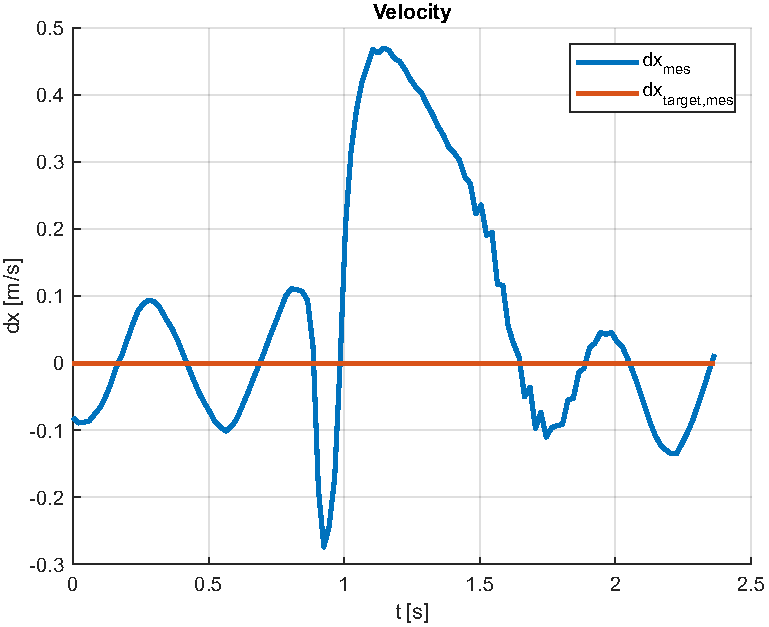
\includegraphics[width=\textwidth]{assets/figures/graphs/hold_positive_speed.pdf}
    \caption{Vitesse lors d'une perturbation positive}
    \label{fig:hold_positive_speed}
\end{figure}

\begin{figure}[H]
    \centering
    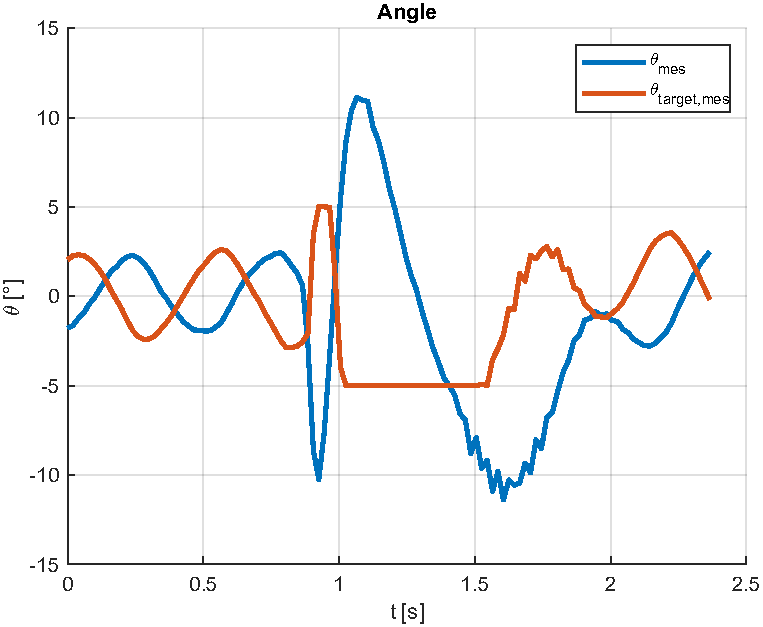
\includegraphics[width=\textwidth]{assets/figures/graphs/hold_positive_angle.pdf}
    \caption{Angle lors d'une perturbation positive}
    \label{fig:hold_positive_angle}
\end{figure}

\begin{figure}[H]
    \centering
    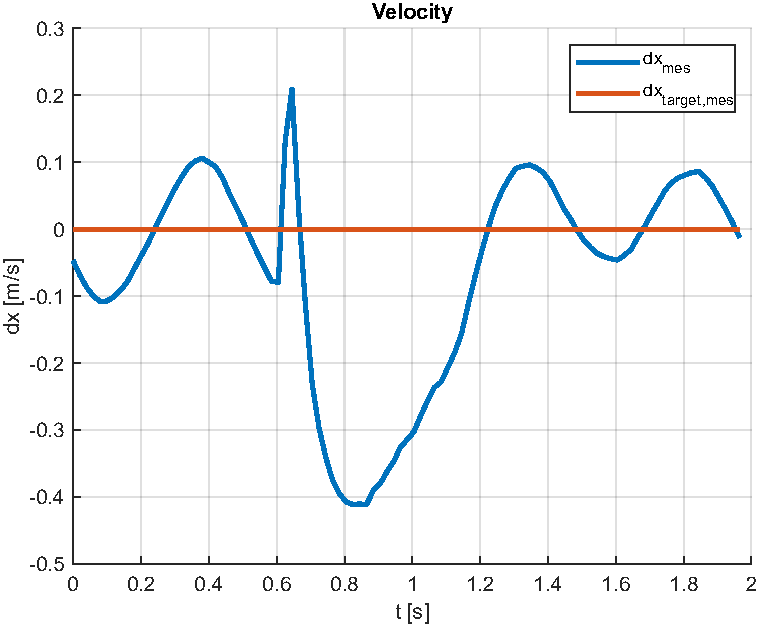
\includegraphics[width=0.8\textwidth]{assets/figures/graphs/hold_negative_speed.pdf}
    \caption{Vitesse lors d'une perturbation négative}
    \label{fig:hold_negative_speed}
\end{figure}

\begin{figure}[H]
    \centering
    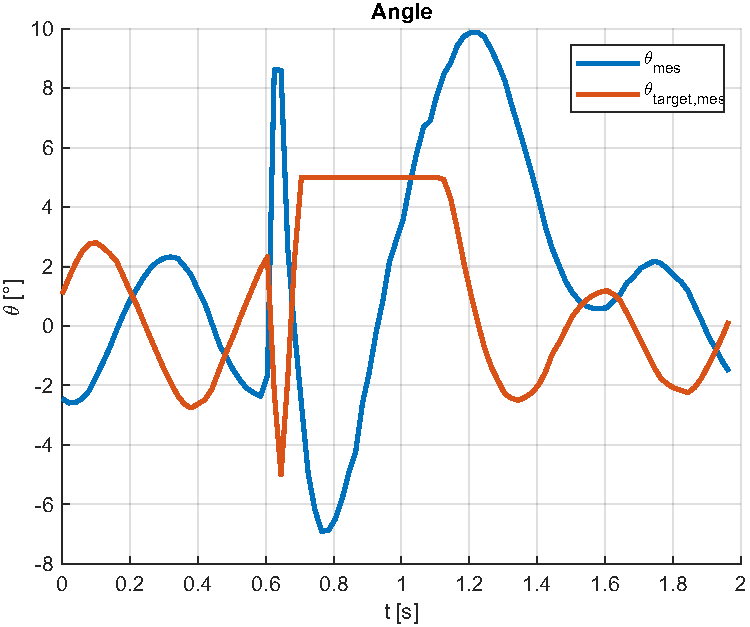
\includegraphics[width=0.8\textwidth]{assets/figures/graphs/hold_negative_angle.pdf}
    \caption{Angle lors d'une perturbation négative}
    \label{fig:hold_negative_angle}
\end{figure}

\subsection{Déplacement trapézoïdal}

Afin d'étudier la capacité de déplacement du système, une loi de vitesse trapézoïdale est utilisée. Ce type de profil permet de limiter les variations brusques de la consigne en imposant une phase d'accélération progressive avant d'atteindre une vitesse constante, puis une phase de décélération avant l'arrêt.

La consigne de vitesse est définie par trois phases successives :

\begin{itemize}
    \item une phase d'accélération durant laquelle la vitesse augmente linéairement jusqu'à atteindre la vitesse maximale ;
    \item une phase à vitesse constante ;
    \item une phase de décélération durant laquelle la vitesse diminue linéairement jusqu'à atteindre une vitesse nulle.
\end{itemize}

La loi de vitesse peut être exprimée sous la forme suivante :

\begin{equation}
v_{ref}(t)=
\begin{cases}
\dfrac{v_{max}}{t_{acc}}t,
& 0\leq t<t_{acc}
\\[10pt]
v_{max},
& t_{acc}\leq t<t_{acc}+t_{c}
\\[10pt]
\dfrac{v_{max}}{t_{dec}}
(t_f-t),
& t_{acc}+t_c\leq t<t_f
\\[10pt]
0,
& t\geq t_f
\end{cases}
\end{equation}


où :
\begin{itemize}
    \item $v_{max}$ correspond à la vitesse maximale demandée ;
    \item $t_{acc}$ représente la durée de la phase d'accélération ;
    \item $t_c$ correspond à la durée de maintien à vitesse constante ;
    \item $t_{dec}$ représente la durée de décélération ;
    \item $t_f$ correspond à la durée totale du déplacement.
\end{itemize}

Dans le cas étudié, la vitesse maximale est fixée à :

\[
v_{max}=0.7\,\mathrm{m/s}
\]

La phase d'accélération dure $2\,\mathrm{s}$, suivie d'une phase à vitesse constante d'une durée de $1\,\mathrm{s}$, puis d'une phase de décélération de $2\,\mathrm{s}$. La durée totale du profil est donc de $5\,\mathrm{s}$.


\begin{figure}[H]
    \centering
    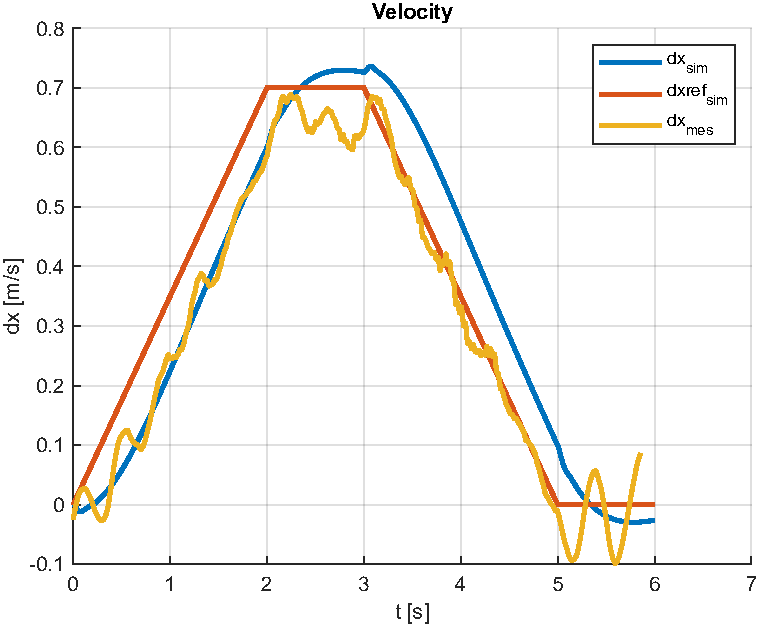
\includegraphics[width=0.8\textwidth]{assets/figures/graphs/trapez_move_velocity.pdf}
    \caption{Évolution de la vitesse lors d'un déplacement trapézoïdal}
    \label{fig:trapez_velocity}
\end{figure}

\begin{figure}[H]
    \centering
    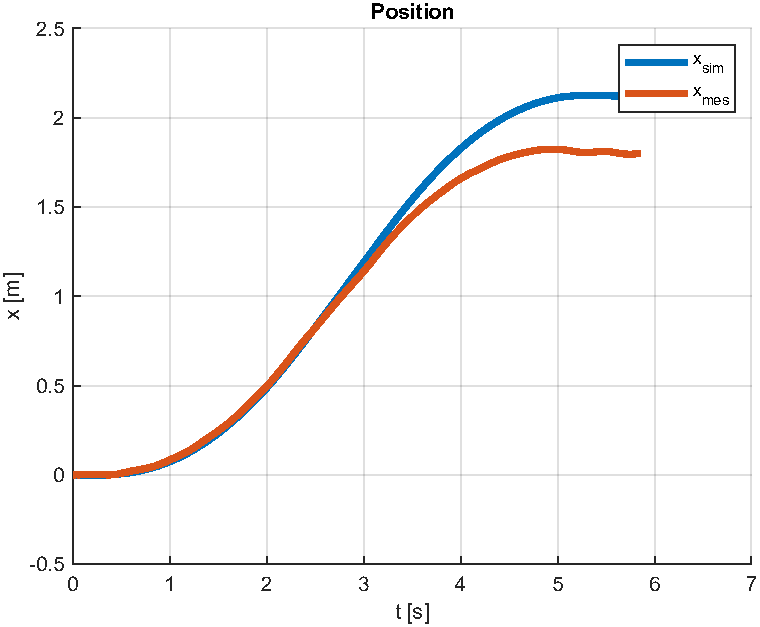
\includegraphics[width=0.8\textwidth]{assets/figures/graphs/trapez_move_position.pdf}
    \caption{Évolution de la position lors d'un déplacement trapézoïdal}
    \label{fig:trapez_position}
\end{figure}


La figure \ref{fig:trapez_velocity} présente l'évolution de la vitesse mesurée. La phase d'accélération suit correctement la rampe imposée par la consigne.

Lors de la phase à vitesse constante, la mesure reste proche de la valeur de consigne $\dot{x} \approx 0.065 \si{\meter\per\second}$. Une différence apparaît toutefois lors de la phase de décélération, durant laquelle la vitesse mesurée diminue plus rapidement que le profil théorique.

La figure \ref{fig:trapez_position} présente l'évolution de la position obtenue à partir du déplacement réalisé. La trajectoire suit globalement la consigne souhaitée. La position finale simulée est de $x_{sim}=2.985\si{\meter}$, tandis que la position mesurée atteint $x_{mes}=2.854\si{\meter}$.

L'écart relatif entre la simulation et la mesure est donné par :

$$
e_x=\frac{|x_{sim}-x_{mes}|}{x_{sim}}\times100
$$

soit :

$$
e_x=\frac{|2.985-2.854|}{2.985}\times100 \approx 4.39\%
$$

\subsection{Impact IMU}

L'impact représente une phase critique pour la mesure, car les accélérations importantes générées lors du contact avec le sol peuvent influencer fortement l'estimation de l'état du système. Cette partie vise à caractériser l'influence de différents paramètres sur le signal mesuré par l'IMU.

\subsubsection{Positionnement}

La position de l'IMU dans la structure influence directement les accélérations mesurées, les raisons de cette influence sont détaillées ici \ref{subsubsection:position_imu}.

La figure \ref{fig:imu_position} présente l'évolution des différents angles mesurés lors du déplacement suivant une loi trapézoïdale présenté précédemment.

On observe que l'angle mesuré par l'IMU suit presque parfaitement l'angle théorique obtenu à partir du modèle physique lors de la phase d'accélération. Ensuite, pour la phase de vitesse constante l'angle revient peu à peu à son angle d'équilibre.

Pour la phase de déceleration, l'angle mesuré par l'IMU est moins important que l'angle simulé, ce dernier reste cependant plus proche de la valeur simulée.

\begin{figure}[H]
    \centering
    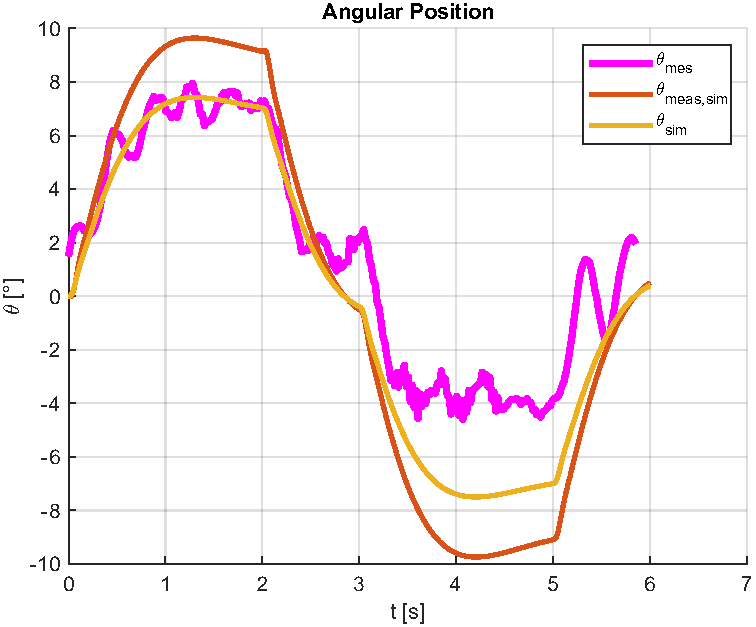
\includegraphics[width=0.8\textwidth]{assets/figures/graphs/trapez_move_theta.pdf}
    \caption{Impact de la position de l'IMU}
    \label{fig:imu_position}
\end{figure}

\subsubsection{Impulsions d'accélération}

Cet essai a pour objectif d'observer l'influence d'une accélération linéaire sur la mesure de l'angle fournie par l'\acrshort{imu}. Pour cela, une perturbation manuelle est appliquée au système en le poussant successivement dans les directions positive et négative.

Les figures \ref{fig:pulse_positive} et \ref{fig:pulse_negative} présentent l'évolution de l'angle mesuré lors de ces perturbations.
 
Tout comme pour la régulation de maintient, l'application d'une accélération à pour effet une lecture de l'angle opposée au sens de poussée.

Les réponses obtenues pour les deux directions de perturbation présentent un comportement similaire avec une inversion du signe de l'évolution de l'angle.

\begin{figure}[H]
    \centering
    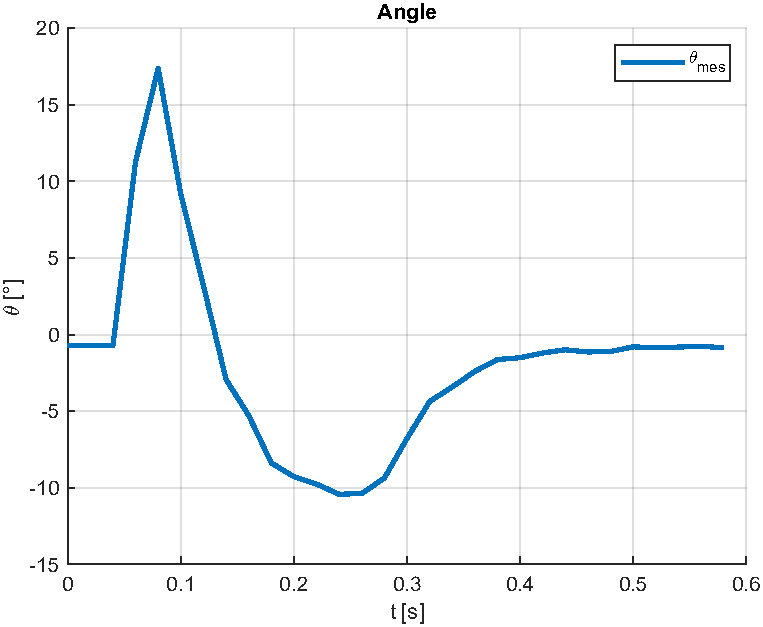
\includegraphics[width=0.8\textwidth]{assets/figures/graphs/pulse_positive.pdf}
    \caption{Variation de l'angle lors d'une accélération positive}
    \label{fig:pulse_positive}
\end{figure}

\begin{figure}[H]
    \centering
    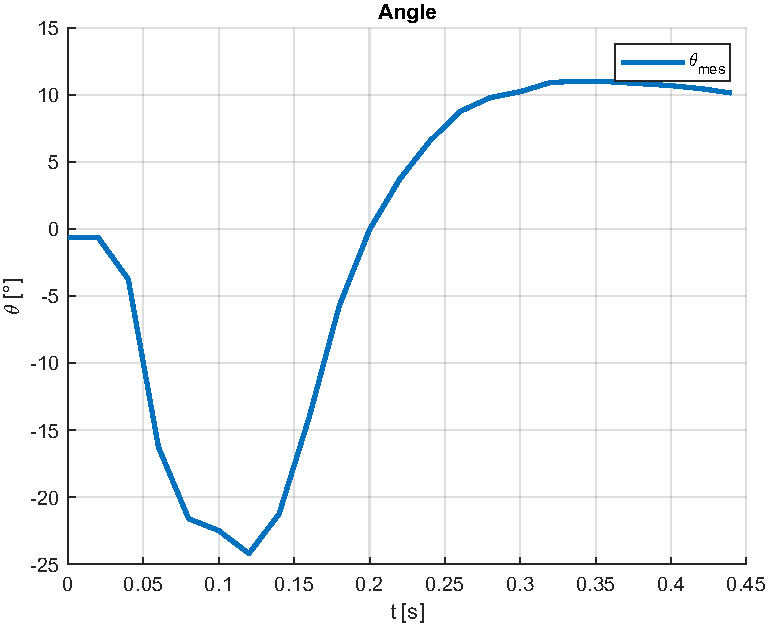
\includegraphics[width=0.8\textwidth]{assets/figures/graphs/pulse_negative.pdf}
    \caption{Impulsion d'accélération négative}
    \label{fig:pulse_negative}
\end{figure}


\section{Electriques}
\subsection{Batterie}
Afin de mesurer le niveau de la batterie, un pont diviseur est utilisé, comme expliqué dans le chapitre consacré à la maquette.

Il est important de s'assurer que les résistances utilisées dans le pont diviseur sont correctement reportées dans le code afin de garantir une lecture fidèle de la tension de la batterie.

\begin{table}[H]
    \centering
    \begin{tabular}{|l|c|c|}
        \hline
        \textbf{Symbole} & \textbf{Valeur théorique} & \textbf{Valeur mesurée} \\
        \hline
        R4 & 10 k$\Omega$ & 10.12 k$\Omega$ \\
        \hline
        R3 & 51 k$\Omega$ & 49.50 k$\Omega$ \\
        \hline
    \end{tabular}
    \caption{Mesure du pont diviseur}
    \label{tab:mesure_pont_diviseur}
\end{table}

 À l'aide des valeurs mesurées, le nouveau rapport du pont diviseur peut être calculé puis introduit dans le code afin d'affiner la mesure de la tension de la batterie.

Le rapport théorique du pont diviseur est donné par :

$$
\frac{R_3+R_4}{R_4}
$$

En utilisant les valeurs mesurées, on obtient :

$$
\frac{50.82 + 10.12}{10.12}=6.022
$$

Le rapport théorique valait :

$$
\frac{51+10}{10}=6.10
$$

On constate donc un écart d'environ (1\%) entre le rapport théorique et le rapport réel.

Il est alors possible de corriger les constantes utilisées dans le programme en remplaçant les valeurs nominales des résistances par les valeurs mesurées :


Le facteur de conversion utilisé pour reconstruire la tension de la batterie devient alors :

$$
\frac{50820+10120}{10120}=6.022
$$

Cette correction permet d'améliorer la précision de la mesure de la tension et de réduire l'erreur introduite par les tolérances des résistances du pont diviseur.

\subsection{Tensions et courants}

Afin d'évaluer la consommation énergétique de la maquette, une mesure du courant total absorbé par le système est réalisée. Pour ce faire, le multimètre est configuré en mode ampèremètre et placé en série entre la batterie et le PCB.

Les tableaux suivants comparent les valeurs théoriques déterminées à la section \ref{section:alimentation} aux mesures expérimentales.

La première mesure est réalisée avec les moteurs désactivés afin de caractériser la consommation électrique des autres modules de la maquette.

\begin{table}[H]
    \centering
    \begin{tabular}{|l|c|c|}
        \hline
        \textbf{Grandeur mesurée} & \textbf{Valeur théorique} & \textbf{Valeur mesurée} \\
        \hline
        $V_{bat}$ & $14.2-16.8\,\si{\volt}$ & $16.20\,\si{\volt}$ \\
        \hline
        $V_{5V}$ & $5.0\,\si{\volt}$ & $5.00\,\si{\volt}$ \\
        \hline
        $V_{IO}$ & $3.3\,\si{\volt}$ & $3.28\,\si{\volt}$ \\
        \hline
        $I_{tot}$ & - & $0.065\,\si{\ampere}$ \\
        \hline
        $P_{tot}$ & $\approx 2\,\si{\watt}$ & $1.05\,\si{\watt}$ \\
        \hline
    \end{tabular}
    \caption{Mesures électriques -- moteurs désactivés}
    \label{tab:moteurs_eteints}
\end{table}

Les tensions mesurées sont très proches des valeurs théoriques. La puissance totale absorbée est de $1.05\,\si{\watt}$, contre une estimation théorique d'environ $2\,\si{\watt}$.

\vspace{0.5cm}

La seconde mesure est réalisée avec les moteurs alimentés mais à vitesse nulle. Dans ce cas, la vitesse angulaire est nulle ($\omega=0$) et la puissance consommée par chaque moteur correspond uniquement aux pertes Joule.

La puissance électrique d'un moteur est donnée par

\begin{equation}
P_{\mathrm{elec}}
=
2I_{\mathrm{RMS}}^{2}R_c
+
T_m\omega.
\end{equation}

Comme $\omega=0$,

\begin{equation}
P_{\mathrm{elec}}
=
2I_{\mathrm{RMS}}^{2}R_c
=
2\times0.81^2\times2.2
=
2.89\,\si{\watt}.
\end{equation}

La puissance totale théorique du système devient alors

\begin{equation}
P_{tot}
=
P_{modules}
+
2P_{\mathrm{elec}}
=
2
+
2\times2.89
=
7.78\,\si{\watt}.
\end{equation}


\begin{table}[H]
    \centering
    \begin{tabular}{|l|c|c|}
        \hline
        \textbf{Grandeur mesurée} & \textbf{Valeur théorique} & \textbf{Valeur mesurée} \\
        \hline
        $V_{bat}$ & $14.2-16.8\,\si{\volt}$ & $16.17\,\si{\volt}$ \\
        \hline
        $V_{5V}$ & $5.0\,\si{\volt}$ & $5.00\,\si{\volt}$ \\
        \hline
        $V_{IO}$ & $3.3\,\si{\volt}$ & $3.28\,\si{\volt}$ \\
        \hline
        $I_{tot}$ & - & $0.195\,\si{\ampere}$ \\
        \hline
        $P_{tot}$ & $7.78\,\si{\watt}$ & $3.15\,\si{\watt}$ \\
        \hline
    \end{tabular}
    \caption{Mesures électriques -- moteurs alimentés, vitesse nulle}
    \label{tab:moteurs_allumes}
\end{table}

La dernière mesure est réalisée lorsque les deux moteurs tournent à la vitesse maximale retenue pour le dimensionnement, soit

\begin{equation}
\omega
=
5\pi
=
15.71\,\si{\radian\per\second}.
\end{equation}

La puissance mécanique développée par un moteur est alors

\begin{equation}
P_{\mathrm{meca}}
=
T_m\omega
=
0.2\times15.71
=
3.14\,\si{\watt}.
\end{equation}

Les pertes Joule restant inchangées,

\begin{equation}
P_{\mathrm{Joule}}
=
2\times0.81^2\times2.2
=
2.89\,\si{\watt},
\end{equation}

la puissance électrique consommée par un moteur devient

\begin{equation}
P_{\mathrm{elec}}
=
P_{\mathrm{Joule}}
+
P_{\mathrm{meca}}
=
2.89
+
3.14
=
6.03\,\si{\watt}.
\end{equation}

La puissance totale théorique du système est donc

\begin{equation}
P_{tot}
=
P_{modules}
+
2P_{\mathrm{elec}}
=
2
+
2\times6.03
=
14.06\,\si{\watt}.
\end{equation}

\begin{table}[H]
    \centering
    \begin{tabular}{|l|c|c|}
        \hline
        \textbf{Grandeur mesurée} & \textbf{Valeur théorique} & \textbf{Valeur mesurée} \\
        \hline
        $V_{bat}$ & $14.2-16.8\,\si{\volt}$ & $16.14\,\si{\volt}$ \\
        \hline
        $V_{5V}$ & $5.0\,\si{\volt}$ & $5.00\,\si{\volt}$ \\
        \hline
        $V_{IO}$ & $3.3\,\si{\volt}$ & $3.28\,\si{\volt}$ \\
        \hline
        $I_{tot}$ & - & $0.551\,\si{\ampere}$ \\
        \hline
        $P_{tot}$ & $14.06\,\si{\watt}$ & $8.89\,\si{\watt}$ \\
        \hline
    \end{tabular}
    \caption{Mesures électriques -- moteurs alimentés à vitesse maximale}
    \label{tab:moteurs_allumes_maxspeed}
\end{table}

\subsection{Autonomie}

L'autonomie de la maquette peut être estimée à partir des consommations mesurées précédemment. Les mesures à vitesse nulle et à vitesse maximale permettent d'encadrer la consommation électrique du système et de fournir une estimation de l'autonomie selon les conditions d'utilisation.
 